\documentclass[letterpaper, 10pt]{article}
\usepackage[margin=0.45in]{geometry}
\usepackage{xifthen}
\usepackage[colorlinks=true,urlcolor=Blue, hidelinks]{hyperref}
\usepackage{graphicx}  % 插图
% \usepackage{cleveref}
\usepackage{newclude}
\usepackage{titlesec}
\usepackage{metalogo}
\usepackage[utf8]{inputenc}
\usepackage[slantfont,boldfont]{xeCJK} % 允许斜体和粗体
\usepackage{kotex}
\usepackage{amsmath, mathrsfs, amsfonts}
\usepackage{tabularray}
\usepackage[dvipsnames]{xcolor}
\usepackage{titling}
\usepackage{titlesec}
\usepackage{minted}
\usepackage{fontawesome5}
\usepackage[customcolors,shade]{hf-tikz}
\usepackage{tkz-euclide}
\usepackage{chngcntr}


\usemintedstyle{xcode}

\newminted{tex}{
  gobble=2,
  linenos,
  mathescape,
  numbersep=5pt,
  frame=single,
  baselinestretch=1.2,
  fontsize=\normalsize,
  highlightcolor=yellow!50,
  highlightlines={},
  breaklines,
}

\definecolor{mygrey}{RGB}{128,128,128}
\definecolor{myteal}{RGB}{0,128,128}
\definecolor{mypink}{RGB}{250,218,221}


\setmainfont{Noto Sans CJK SC}
\setCJKmainfont{Noto Sans CJK SC}
\setCJKsansfont{Noto Sans CJK SC}
\setCJKmonofont{Noto Sans CJK SC}

\NewTableCommand\myhline{\hline[0.2em,black]}


\let\oldhref\href
\renewcommand{\href}[3][blue]{\oldhref{#2}{\color{#1}{#3}}}


% Link images
\newcommand{\pdf}{
\includegraphics[height=.85em]{png/pdf.png}}
\newcommand{\gh}{
\includegraphics[height=.85em]{png/gh.png}}
\newcommand{\www}{
\includegraphics[height=.85em]{png/www.png}}
\newcommand{\email}{
\includegraphics[height=.85em]{png/email.png}}
\newcommand{\yt}{
\includegraphics[height=.85em]{png/yt.png}}
\newcommand{\gitee}{
\includegraphics[height=.85em]{png/gitee.png}}

% \title{Constructing a Nuclear Reactor Using Only Coconuts}
\author{LcdSe7en}
\date{\today}


% Custom title command.
\renewcommand{\maketitle}{
	\hspace{.25\textwidth}
	\begin{minipage}[t]{.5\textwidth}
    \par{\centering{\Huge  \texttt{\theauthor}}\par}
	\end{minipage}
	\begin{minipage}[t]{.25\textwidth}
   {\footnotesize\hfill{}\color{gray}
     \hfill{}Download this document:

     \hfill{}\href[gray]{https://github.com/lcdse7en/archlinux}{documents.pdf \pdf}

     \hfill{}(Last updated \thedate.)
    }
	\end{minipage}
}

% -----------------------------------------
% ---   Setting Table Environment Begin ---
% -----------------------------------------
\NewTblrEnviron{mytblr}
\SetTblrOuter[mytblr]{long}
\SetTblrInner[mytblr]{
  width = 0.99\linewidth,
  rowhead = 1,
  verb,
  row{odd} = {bg=mypink}, 
  row{1}   = {bg=myteal, fg=white},
}
\SetTblrStyle{caption-tag}{red2}
\SetTblrStyle{firstfoot}{fg=blue2}
\SetTblrStyle{firsthead}{font=\bfseries}

\UseTblrLibrary{counter}
\newcounter{mycnta}
\newcommand{\mycnta}{\stepcounter{mycnta}\arabic{mycnta}}
\counterwithin{mycnta}{page}  % 换页重新关联排序
\renewcommand\themycnta{\arabic{mycnta}}
% ---   Setting Table Environment end ---

\titleformat{\section}{\Large\bf\raggedright}{}{1em}{}[{\titlerule[2pt]}]

\begin{document}

\maketitle


\begin{minipage}[t]{.5\linewidth}
\begin{tabular}{rp{.75\linewidth}}
	\baselineskip=20pt
	\email{} :     & \href{2353442022@qq.com}{2353442022@qq.com}\\
	\www{} : &\href{https://texdoc.org/index.html}{https://texdoc.org/index.html}
\end{tabular}
\end{minipage}
\begin{minipage}[t]{.5\linewidth}
\begin{tabular}{rl}
	\gh{} : & \href{https://github.com/lcdse7en/latex-packages}{https://github.com/lcdse7en/latex-packages}\\
	\gitee{} : &\href{https://gitee.com/se7enlcd}{https://gitee.com/se7enlcd}
\end{tabular}
\end{minipage}

\include*{documents/packages-table} % 不分页
\section{Start Use and Setting package \textcolor{green}{\faIcon{github}} \textcolor{blue}{\faIcon{code}} \faIcon{university} \textcolor{cyan}{\faIcon{google-plus}} \faIcon{at}}


\begin{minted}[
  encoding=utf8,
  linenos,
  gobble=2,
  mathescape,
  numbersep=5pt,
  frame=single,
  framesep=2mm,
  baselinestretch=1.2,
  fontsize=\normalsize, % huge, LARGE, large, normalsize, small, footnotesize, scriptsize
  highlightcolor=cyan!50,
  breaklines]{tex}
  \documentclass[letterpaper, 10pt]{article}
  \usepackage[slantfont,boldfont]{xeCJK}
  \usepackage{kotex} % Korea language environment
  \usepackage[margin=0.45in]{geometry}
  \usepackage{metalogo}
  \usepackage[dvipsnames]{xcolor}
  \usepackage[colorlinks=true,urlcolor=Blue]{hyperref}
  \usepackage{titling}
  \usepackage{newclude} % page break

  % ------------------------ Set language ---------------------------
  \setmainfont{Noto Sans CJK SC}
  \setCJKmainfont{Noto Sans CJK SC}
  \setCJKsansfont{Noto Sans CJK SC}
  \setCJKmonofont{Noto Sans CJK SC}

  % ------------------- Link images Begin ---------------------------
  \newcommand{\pdf}{
\includegraphics[height=.85em]{png/pdf.png}}
  \newcommand{\gh}{
\includegraphics[height=.85em]{png/gh.png}}
  \newcommand{\www}{
\includegraphics[height=.85em]{png/www.png}}
  \newcommand{\email}{
\includegraphics[height=.85em]{png/email.png}}
  \newcommand{\yt}{
\includegraphics[height=.85em]{png/yt.png}}
  \newcommand{\gitee}{
\includegraphics[height=.85em]{png/gitee.png}}

  % ------------------ Custom title command. ------------------------
  \renewcommand{\maketitle}{
    \hspace{.25\textwidth}
    \begin{minipage}[t]{.5\textwidth}
      \par{\centering{\Huge  \texttt{\theauthor}}\par}
    \end{minipage}
    \begin{minipage}[t]{.25\textwidth}
     {\footnotesize\hfill{}\color{gray}
       \hfill{}Download this document:

       \hfill{}\href[gray]{https://github.com/lcdse7en/archlinux}{documents.pdf \pdf}

       \hfill{}(Last updated \thedate.)
      }
    \end{minipage}
  }

  \let\oldhref\href
  \renewcommand{\href}[3][blue]{\oldhref{#2}{\color{#1}{#3}}}
  
  \author{LcdSe7en}
  \date{\today}

\end{minted}

\newpage

\section{Begin document \textcolor{green}{\faIcon{github}} \textcolor{blue}{\faIcon{code}} \faIcon{university} \textcolor{cyan}{\faIcon{google-plus}} \faIcon{at}}
\begin{minted}[
  encoding=utf8,
  linenos,
  gobble=2,
  mathescape,
  numbersep=5pt,
  frame=single,
  framesep=2mm,
  baselinestretch=1.2,
  fontsize=\normalsize, % huge, LARGE, large, normalsize, small, footnotesize, scriptsize
  highlightcolor=cyan!50,
  breaklines]{vim}
  nnoremap <buffer> <F6> <cmd>ToggleTerm size=10 direction=horizontal<cr><cmd>terminal latexmk -pvc *.tex<cr>A
  nnoremap <buffer> <F7> <cmd>ToggleTerm size=10 direction=horizontal<cr><cmd>terminal latexmk -pvc --shell-escape *.tex<cr>A
\end{minted}

\begin{figure}[hbt!]
\centering
\begin{minipage}{0.95\textwidth}
  \centering
  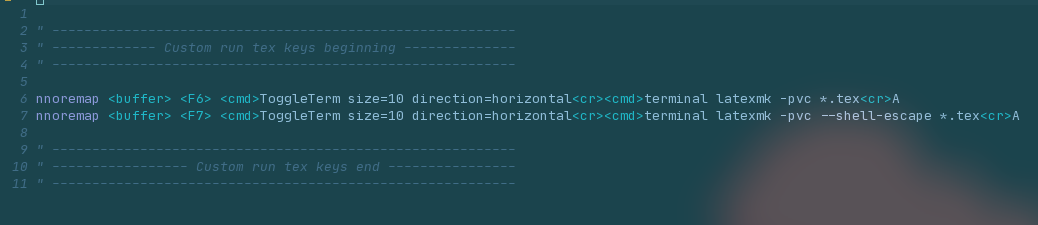
\includegraphics[width=\textwidth]{images/key.png}
\end{minipage}
\end{figure}

\begin{minted}[
  encoding=utf8,
  linenos,
  gobble=2,
  mathescape,
  numbersep=5pt,
  frame=single,
  framesep=2mm,
  baselinestretch=1.2,
  fontsize=\normalsize, % huge, LARGE, large, normalsize, small, footnotesize, scriptsize
  highlightcolor=cyan!50,
  breaklines]{tex}
  \begin{document}

  \maketitle

  \begin{minipage}[t]{.5\linewidth}
  \begin{tabular}{rp{.75\linewidth}}
    \baselineskip=20pt
    \email{} :  &\href{2353442022@qq.com}{2353442022@qq.com}\\
    \www{} :    &\href{https://github.com/lcdse7en/latex-packages}{https://github.com/lcdse7en/latex-packages}
  \end{tabular}
  \end{minipage}
  \begin{minipage}[t]{.5\linewidth}
  \begin{tabular}{rl}
    \gh{} :    &\href{https://github.com/lcdse7en}{https://github.com/lcdse7en}\\
    \gitee{} : &\href{https://gitee.com/se7enlcd}{https://gitee.com/se7enlcd}
  \end{tabular}
  \end{minipage}


  % no page break
  % \usepackage{newclude}
  \include*{documents/packages-table}

  \section{Start Use and Setting package \textcolor{green}{\faIcon{github}} \textcolor{blue}{\faIcon{code}} \faIcon{university} \textcolor{cyan}{\faIcon{google-plus}} \faIcon{at}}


\begin{minted}[
  encoding=utf8,
  linenos,
  gobble=2,
  mathescape,
  numbersep=5pt,
  frame=single,
  framesep=2mm,
  baselinestretch=1.2,
  fontsize=\normalsize, % huge, LARGE, large, normalsize, small, footnotesize, scriptsize
  highlightcolor=cyan!50,
  breaklines]{tex}
  \documentclass[letterpaper, 10pt]{article}
  \usepackage[slantfont,boldfont]{xeCJK}
  \usepackage{kotex} % Korea language environment
  \usepackage[margin=0.45in]{geometry}
  \usepackage{metalogo}
  \usepackage[dvipsnames]{xcolor}
  \usepackage[colorlinks=true,urlcolor=Blue]{hyperref}
  \usepackage{titling}
  \usepackage{newclude} % page break

  % ------------------------ Set language ---------------------------
  \setmainfont{Noto Sans CJK SC}
  \setCJKmainfont{Noto Sans CJK SC}
  \setCJKsansfont{Noto Sans CJK SC}
  \setCJKmonofont{Noto Sans CJK SC}

  % ------------------- Link images Begin ---------------------------
  \newcommand{\pdf}{
\includegraphics[height=.85em]{png/pdf.png}}
  \newcommand{\gh}{
\includegraphics[height=.85em]{png/gh.png}}
  \newcommand{\www}{
\includegraphics[height=.85em]{png/www.png}}
  \newcommand{\email}{
\includegraphics[height=.85em]{png/email.png}}
  \newcommand{\yt}{
\includegraphics[height=.85em]{png/yt.png}}
  \newcommand{\gitee}{
\includegraphics[height=.85em]{png/gitee.png}}

  % ------------------ Custom title command. ------------------------
  \renewcommand{\maketitle}{
    \hspace{.25\textwidth}
    \begin{minipage}[t]{.5\textwidth}
      \par{\centering{\Huge  \texttt{\theauthor}}\par}
    \end{minipage}
    \begin{minipage}[t]{.25\textwidth}
     {\footnotesize\hfill{}\color{gray}
       \hfill{}Download this document:

       \hfill{}\href[gray]{https://github.com/lcdse7en/archlinux}{documents.pdf \pdf}

       \hfill{}(Last updated \thedate.)
      }
    \end{minipage}
  }

  \let\oldhref\href
  \renewcommand{\href}[3][blue]{\oldhref{#2}{\color{#1}{#3}}}
  
  \author{LcdSe7en}
  \date{\today}

\end{minted}

\newpage

\section{Begin document \textcolor{green}{\faIcon{github}} \textcolor{blue}{\faIcon{code}} \faIcon{university} \textcolor{cyan}{\faIcon{google-plus}} \faIcon{at}}
\begin{minted}[
  encoding=utf8,
  linenos,
  gobble=2,
  mathescape,
  numbersep=5pt,
  frame=single,
  framesep=2mm,
  baselinestretch=1.2,
  fontsize=\normalsize, % huge, LARGE, large, normalsize, small, footnotesize, scriptsize
  highlightcolor=cyan!50,
  breaklines]{vim}
  nnoremap <buffer> <F6> <cmd>ToggleTerm size=10 direction=horizontal<cr><cmd>terminal latexmk -pvc *.tex<cr>A
  nnoremap <buffer> <F7> <cmd>ToggleTerm size=10 direction=horizontal<cr><cmd>terminal latexmk -pvc --shell-escape *.tex<cr>A
\end{minted}

\begin{figure}[hbt!]
\centering
\begin{minipage}{0.95\textwidth}
  \centering
  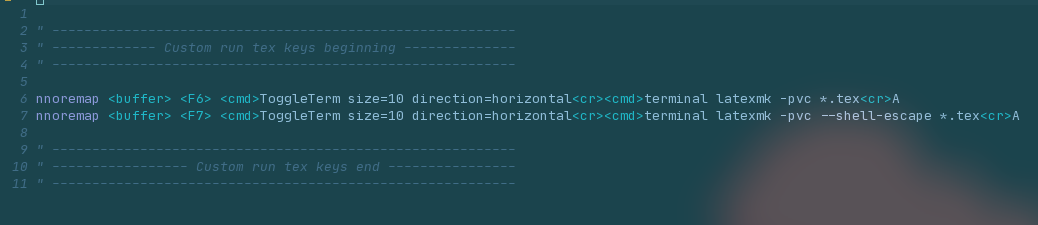
\includegraphics[width=\textwidth]{images/key.png}
\end{minipage}
\end{figure}

\begin{minted}[
  encoding=utf8,
  linenos,
  gobble=2,
  mathescape,
  numbersep=5pt,
  frame=single,
  framesep=2mm,
  baselinestretch=1.2,
  fontsize=\normalsize, % huge, LARGE, large, normalsize, small, footnotesize, scriptsize
  highlightcolor=cyan!50,
  breaklines]{tex}
  \begin{document}

  \maketitle

  \begin{minipage}[t]{.5\linewidth}
  \begin{tabular}{rp{.75\linewidth}}
    \baselineskip=20pt
    \email{} :  &\href{2353442022@qq.com}{2353442022@qq.com}\\
    \www{} :    &\href{https://github.com/lcdse7en/latex-packages}{https://github.com/lcdse7en/latex-packages}
  \end{tabular}
  \end{minipage}
  \begin{minipage}[t]{.5\linewidth}
  \begin{tabular}{rl}
    \gh{} :    &\href{https://github.com/lcdse7en}{https://github.com/lcdse7en}\\
    \gitee{} : &\href{https://gitee.com/se7enlcd}{https://gitee.com/se7enlcd}
  \end{tabular}
  \end{minipage}


  % no page break
  % \usepackage{newclude}
  \include*{documents/packages-table}

  \section{Start Use and Setting package \textcolor{green}{\faIcon{github}} \textcolor{blue}{\faIcon{code}} \faIcon{university} \textcolor{cyan}{\faIcon{google-plus}} \faIcon{at}}


\begin{minted}[
  encoding=utf8,
  linenos,
  gobble=2,
  mathescape,
  numbersep=5pt,
  frame=single,
  framesep=2mm,
  baselinestretch=1.2,
  fontsize=\normalsize, % huge, LARGE, large, normalsize, small, footnotesize, scriptsize
  highlightcolor=cyan!50,
  breaklines]{tex}
  \documentclass[letterpaper, 10pt]{article}
  \usepackage[slantfont,boldfont]{xeCJK}
  \usepackage{kotex} % Korea language environment
  \usepackage[margin=0.45in]{geometry}
  \usepackage{metalogo}
  \usepackage[dvipsnames]{xcolor}
  \usepackage[colorlinks=true,urlcolor=Blue]{hyperref}
  \usepackage{titling}
  \usepackage{newclude} % page break

  % ------------------------ Set language ---------------------------
  \setmainfont{Noto Sans CJK SC}
  \setCJKmainfont{Noto Sans CJK SC}
  \setCJKsansfont{Noto Sans CJK SC}
  \setCJKmonofont{Noto Sans CJK SC}

  % ------------------- Link images Begin ---------------------------
  \newcommand{\pdf}{
\includegraphics[height=.85em]{png/pdf.png}}
  \newcommand{\gh}{
\includegraphics[height=.85em]{png/gh.png}}
  \newcommand{\www}{
\includegraphics[height=.85em]{png/www.png}}
  \newcommand{\email}{
\includegraphics[height=.85em]{png/email.png}}
  \newcommand{\yt}{
\includegraphics[height=.85em]{png/yt.png}}
  \newcommand{\gitee}{
\includegraphics[height=.85em]{png/gitee.png}}

  % ------------------ Custom title command. ------------------------
  \renewcommand{\maketitle}{
    \hspace{.25\textwidth}
    \begin{minipage}[t]{.5\textwidth}
      \par{\centering{\Huge  \texttt{\theauthor}}\par}
    \end{minipage}
    \begin{minipage}[t]{.25\textwidth}
     {\footnotesize\hfill{}\color{gray}
       \hfill{}Download this document:

       \hfill{}\href[gray]{https://github.com/lcdse7en/archlinux}{documents.pdf \pdf}

       \hfill{}(Last updated \thedate.)
      }
    \end{minipage}
  }

  \let\oldhref\href
  \renewcommand{\href}[3][blue]{\oldhref{#2}{\color{#1}{#3}}}
  
  \author{LcdSe7en}
  \date{\today}

\end{minted}

\newpage

\section{Begin document \textcolor{green}{\faIcon{github}} \textcolor{blue}{\faIcon{code}} \faIcon{university} \textcolor{cyan}{\faIcon{google-plus}} \faIcon{at}}
\begin{minted}[
  encoding=utf8,
  linenos,
  gobble=2,
  mathescape,
  numbersep=5pt,
  frame=single,
  framesep=2mm,
  baselinestretch=1.2,
  fontsize=\normalsize, % huge, LARGE, large, normalsize, small, footnotesize, scriptsize
  highlightcolor=cyan!50,
  breaklines]{vim}
  nnoremap <buffer> <F6> <cmd>ToggleTerm size=10 direction=horizontal<cr><cmd>terminal latexmk -pvc *.tex<cr>A
  nnoremap <buffer> <F7> <cmd>ToggleTerm size=10 direction=horizontal<cr><cmd>terminal latexmk -pvc --shell-escape *.tex<cr>A
\end{minted}

\begin{figure}[hbt!]
\centering
\begin{minipage}{0.95\textwidth}
  \centering
  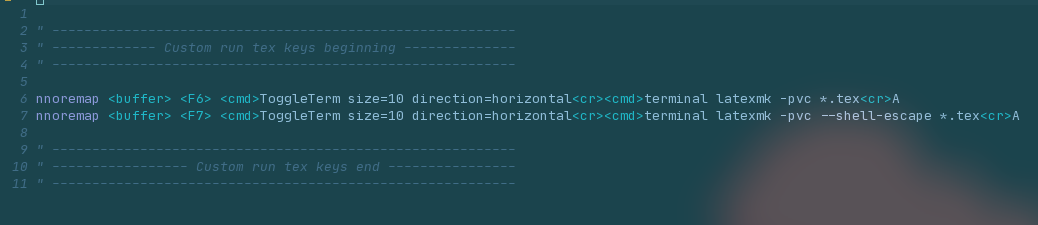
\includegraphics[width=\textwidth]{images/key.png}
\end{minipage}
\end{figure}

\begin{minted}[
  encoding=utf8,
  linenos,
  gobble=2,
  mathescape,
  numbersep=5pt,
  frame=single,
  framesep=2mm,
  baselinestretch=1.2,
  fontsize=\normalsize, % huge, LARGE, large, normalsize, small, footnotesize, scriptsize
  highlightcolor=cyan!50,
  breaklines]{tex}
  \begin{document}

  \maketitle

  \begin{minipage}[t]{.5\linewidth}
  \begin{tabular}{rp{.75\linewidth}}
    \baselineskip=20pt
    \email{} :  &\href{2353442022@qq.com}{2353442022@qq.com}\\
    \www{} :    &\href{https://github.com/lcdse7en/latex-packages}{https://github.com/lcdse7en/latex-packages}
  \end{tabular}
  \end{minipage}
  \begin{minipage}[t]{.5\linewidth}
  \begin{tabular}{rl}
    \gh{} :    &\href{https://github.com/lcdse7en}{https://github.com/lcdse7en}\\
    \gitee{} : &\href{https://gitee.com/se7enlcd}{https://gitee.com/se7enlcd}
  \end{tabular}
  \end{minipage}


  % no page break
  % \usepackage{newclude}
  \include*{documents/packages-table}

  \include{documents/start}
  \include{documents/fontawesome5}
  \include{documents/graphicx}
  \include{documents/minted}
  \include{documents/tabularray}

  \end{document}
\end{minted}

\newpage

  

\section{fontawesome5 \textcolor{green}{\faIcon{github}} \textcolor{blue}{\faIcon{code}} \faIcon{university} \textcolor{cyan}{\faIcon{google-plus}} \faIcon{at}}

\begin{minipage}[t]{.5\linewidth}
\begin{tabular}{rp{.75\linewidth}}
	\baselineskip=20pt
	\email{} :     & \href{2353442022@qq.com}{2353442022@qq.com}\\
	\www{} : &\href{https://fontawesome.com/v5/search}{https://fontawesome.com/v5/search}
\end{tabular}
\end{minipage}
\begin{minipage}[t]{.5\linewidth}
\begin{tabular}{rl}
	\gh{} : & \href{https://github.com/lcdse7en}{https://github.com/lcdse7en}\\
	\gitee{} : &\href{https://gitee.com/se7enlcd}{https://gitee.com/se7enlcd}
\end{tabular}
\end{minipage}

\begin{minted}[
  encoding=utf8,
  linenos,
  gobble=2,
  mathescape,
  numbersep=5pt,
  frame=single,
  framesep=2mm,
  baselinestretch=1.2,
  fontsize=\normalsize, % huge, LARGE, large, normalsize, small, footnotesize, scriptsize
  highlightcolor=cyan!50,
  highlightlines={6,8},
  breaklines]{tex}
  \documentclass[letterpaper, 10pt]{article}
  \usepackage{fontawesome5}

  \begin{document}

  \faIcon{tint}

  \textcolor{red}{\faIcon{tint}}

  \end{document}

\end{minted}


\begin{mytblr}[
    caption = {Fontawesome5 Icons},
  ]{
    colspec={|l|X[2.8]|X[2.8]|l|X[2.8]|X[2.8]|X[2.8]|},
    }
    \myhline
    \SetRow{c} ID & Icon Name & Show            & ID         & Icon Name    & Show                  \\
    \myhline
    \mycnta & yin-yang    & \faIcon{yin-yang}     & \mycnta    & transgender  & \faIcon{transgender}  \\
    \mycnta & yen-sign    & \faIcon{yen-sign}     & \mycnta    & toggle-on    & \faIcon{toggle-on}    \\
    \mycnta & video       & \faIcon{video}        & \mycnta    & terminal     & \faIcon{terminal}     \\
    \mycnta & user-secret & \faIcon{user-secret}  & \mycnta    & tag          & \faIcon{tag}          \\
    \mycnta & store       & \faIcon{store}        & \mycnta    & share        & \faIcon{share}       \\
    \mycnta & phone-volume& \faIcon{phone-volume} & \mycnta    & pen-nib      & \faIcon{pen-nib}     \\
    \mycnta & smoking-ban & \faIcon{smoking-ban}  & \mycnta    & magnet       & \faIcon{magnet}      \\
    \mycnta & smoking     & \faIcon{smoking}      & \mycnta    & landmark     & \faIcon{landmark}    \\
    \mycnta & id-card     & \faIcon{id-card}    & \mycnta      & heart        & \faIcon{heart}       \\
    \mycnta & code     & \faIcon{code}    & \mycnta      & clock        & \faIcon{clock}       \\
    \mycnta & clone     & \faIcon{clone}    & \mycnta      & check        & \faIcon{check}       \\
    \mycnta & youtube     & \faIcon{youtube}    & \mycnta      & weixin        & \faIcon{weixin}       \\
    \mycnta & weibo     & \faIcon{weibo}    & \mycnta      & whatsapp        & \faIcon{whatsapp}       \\
    \mycnta & python     & \faIcon{python}    & \mycnta      & qq        & \faIcon{qq}       \\
    \mycnta & google-plus     & \faIcon{google-plus}    & \mycnta      & github        & \faIcon{github}       \\
    \mycnta & chrome     & \faIcon{chrome}    & \mycnta      & tint        & \faIcon{tint}       \\
    \mycnta & chart-line     & \faIcon{chart-line}    & \mycnta      &         &        \\
    \mycnta &             &             & \mycnta      &         &        \\
    \mycnta &             &             & \mycnta      &         &        \\
    \mycnta &             &             & \mycnta      &         &        \\
    \mycnta &             &             & \mycnta      &         &        \\
    \mycnta &             &             & \mycnta      &         &        \\
    \mycnta &             &             & \mycnta      &         &        \\
    \mycnta &             &             & \mycnta      &         &        \\
    \mycnta &             &             & \mycnta      &         &        \\
    \myhline 
\end{mytblr}

\newpage

  \section{graphicx \textcolor{green}{\faIcon{github}} \textcolor{blue}{\faIcon{code}} \faIcon{university} \textcolor{cyan}{\faIcon{google-plus}} \faIcon{at}}


\begin{minted}[
  encoding=utf8,
  linenos,
  gobble=2,
  mathescape,
  numbersep=5pt,
  frame=single,
  framesep=2mm,
  baselinestretch=1.2,
  fontsize=\normalsize, % huge, LARGE, large, normalsize, small, footnotesize, scriptsize
  highlightcolor=cyan!50,
  highlightlines={7,12},
  breaklines]{tex}
  \usepackage{graphicx}

  \begin{figure}[hbt!]
  \centering
  \begin{minipage}{0.49\textwidth}
    \centering
    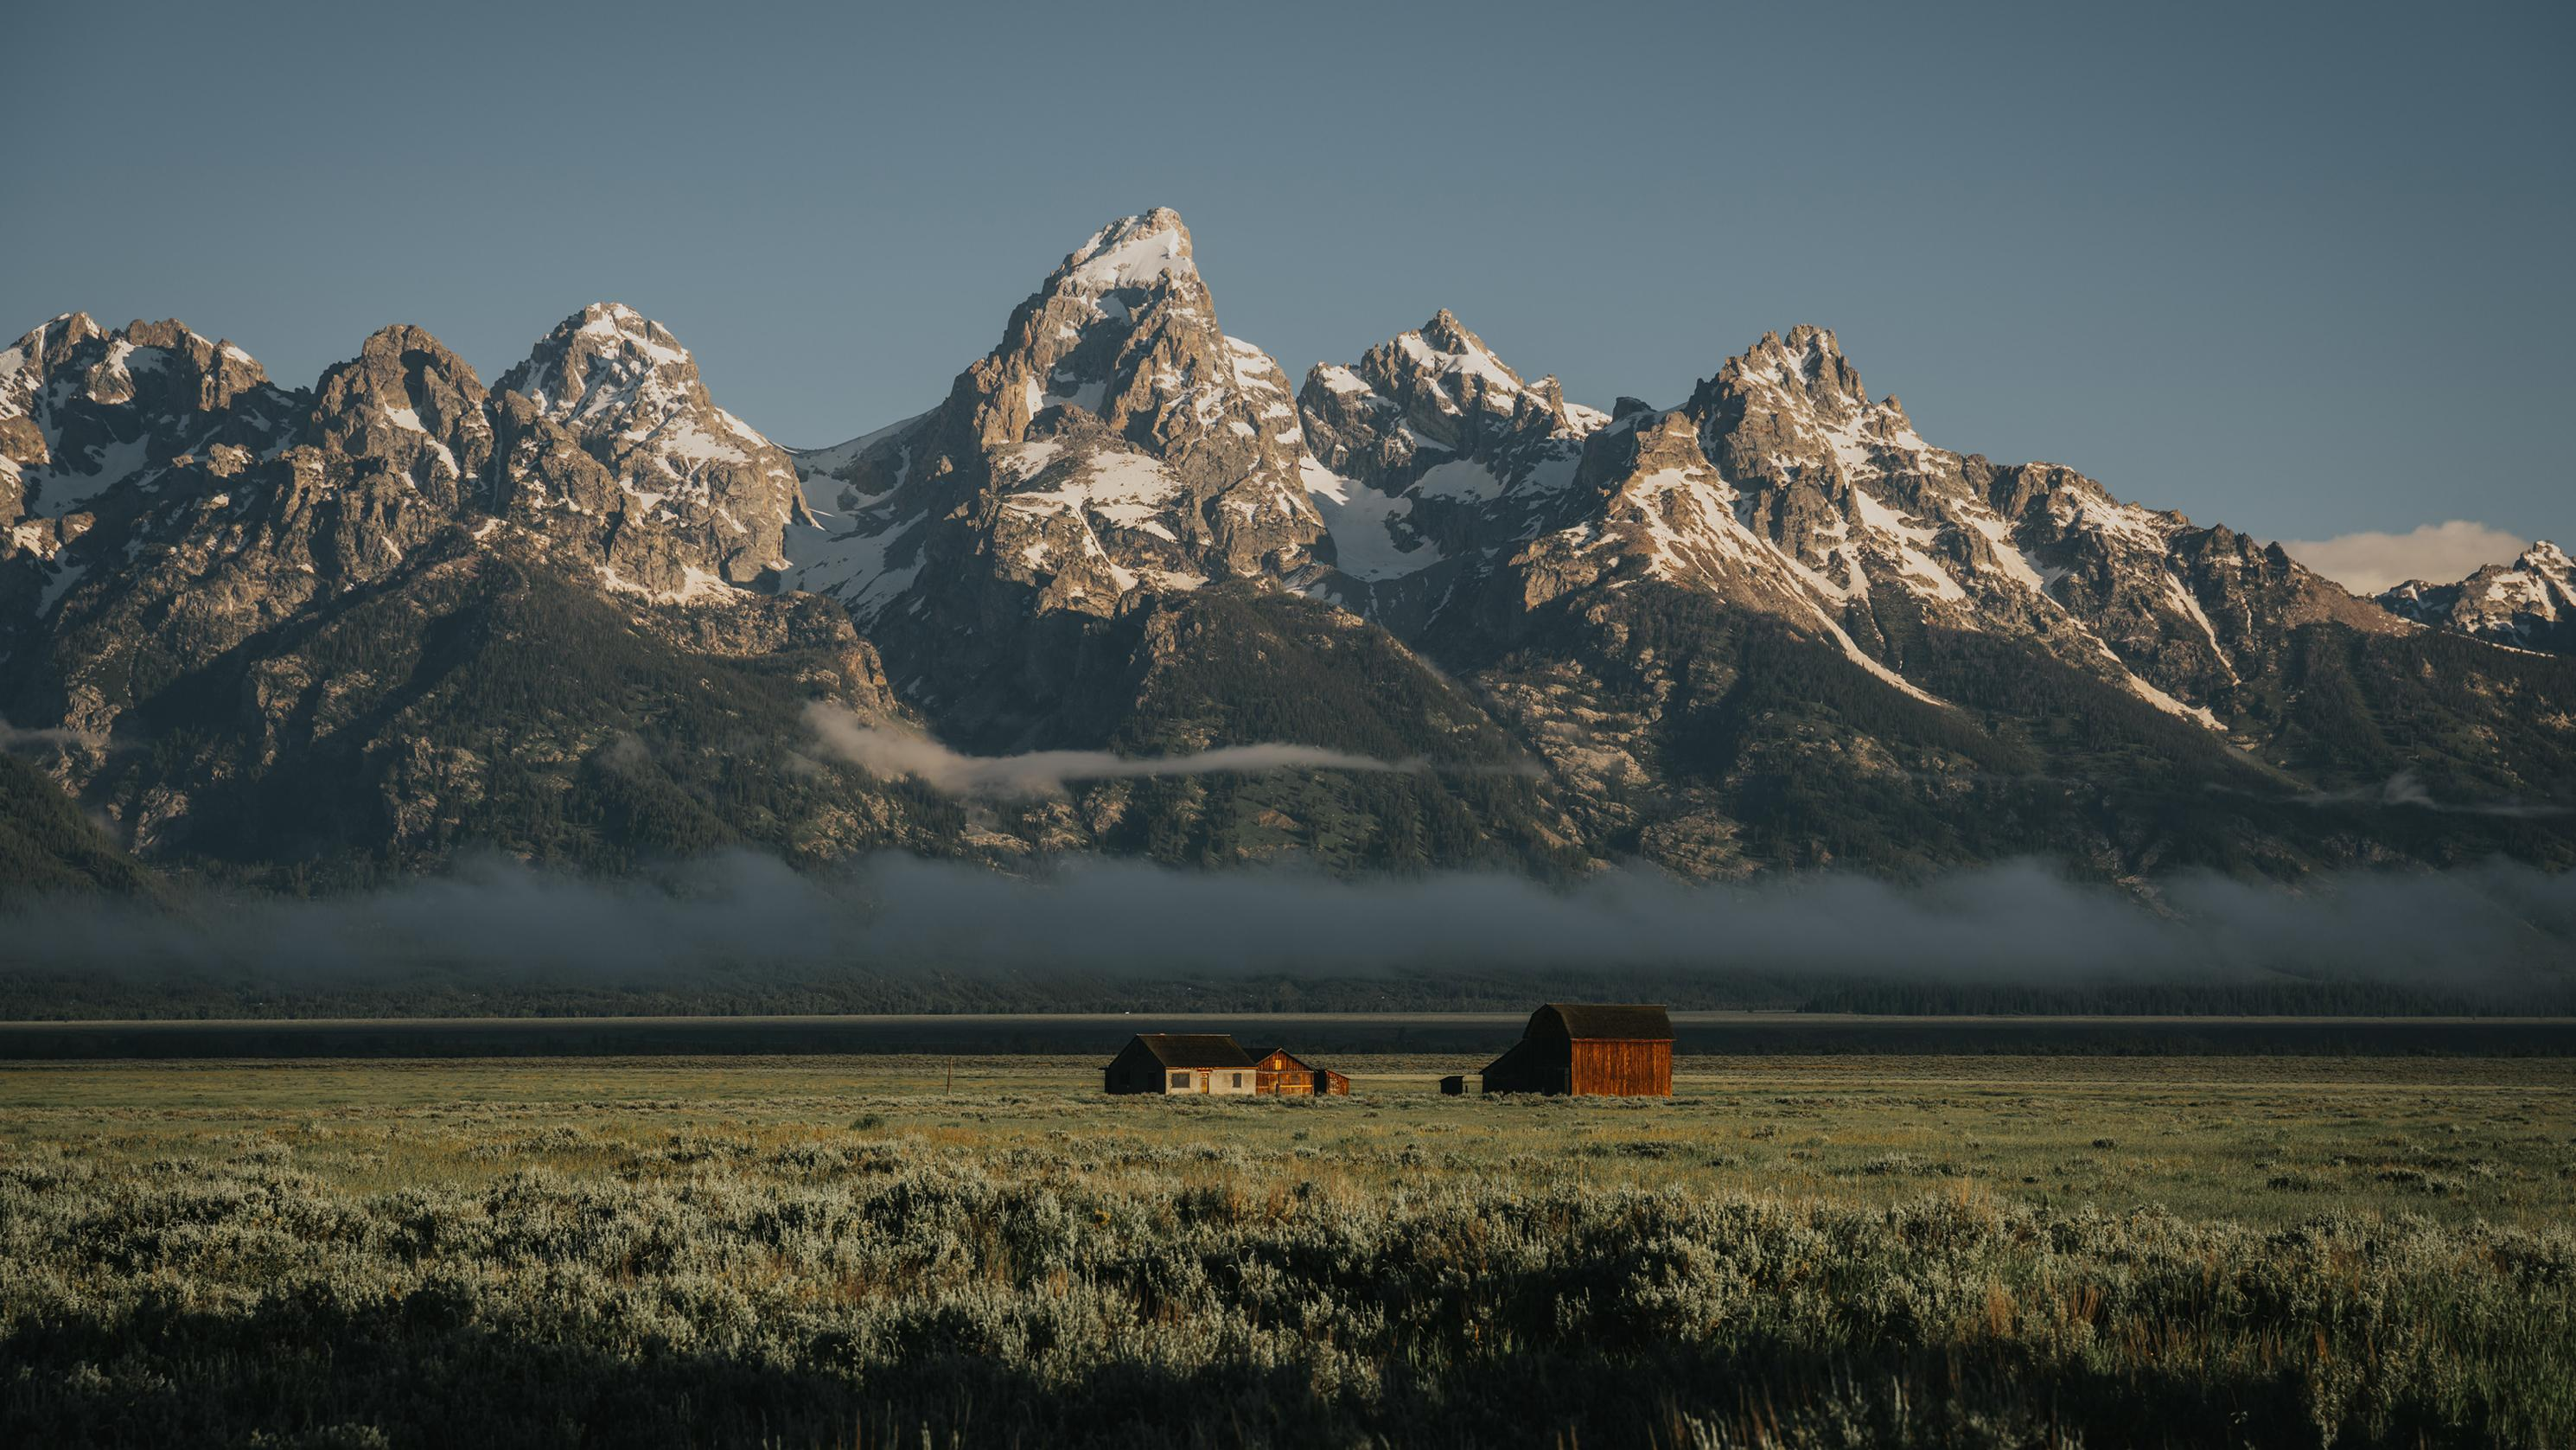
\includegraphics[width=\textwidth]{images/1.jpg}
    \caption{1}
  \end{minipage}
  \begin{minipage}{0.49\textwidth}
    \centering
    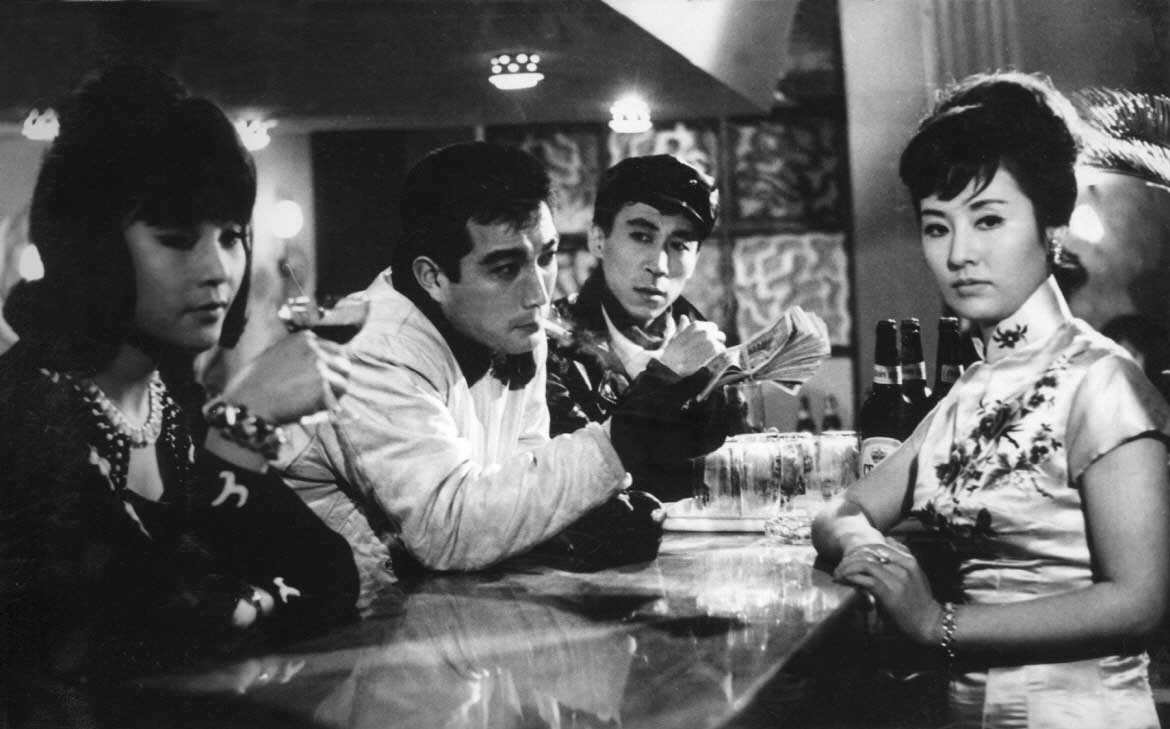
\includegraphics[width=\textwidth]{images/2.jpg}
    \caption{2}
  \end{minipage}
  \end{figure}
\end{minted}


\newpage

  
\section{minted  \textcolor{green}{\faIcon{github}} \textcolor{blue}{\faIcon{code}} \faIcon{university} \textcolor{cyan}{\faIcon{google-plus}} \faIcon{at}}

\begin{texcode}
  % sudo pip3 install pygments
  % -shell-escape

  \documentclass[letterpaper, 10pt]{article}
  \usepackage{minted}
  \usepackage{xcolor}
  \usepackage{fontawesome5} % \textcolor{green}{\faIcon{github}}

  \usemintedstyle{xcode} % pygmentize -L styles [xcode, github-dark]
  

  % Custom Code Environments
  \newminted{tex}{
    gobble=2,
    linenos,
    mathescape,
    numbersep=5pt,
    frame=single,
    baselinestretch=1.2,
    fontsize=\normalsize, % huge, LARGE, large, normalsize, small, footnotesize, scriptsize, tiny
    highlightcolor=yellow!50,
    highlightlines={1,3},
    bgcolor=bg,
    breaklines,
  }

  \begin{document}

  % \begin{Customcode}
  \begin{minted}[
      encoding=utf8,
      linenos,
      gobble=2,
      mathescape,
      numbersep=5pt,
      frame=single,
      framesep=2mm,
      baselinestretch=1.2,
      fontsize=\large, % huge, LARGE, large, normalsize, small, footnotesize, scriptsize, tiny
      highlightcolor=yellow!50,
      highlightlines={1,3},
      bgcolor=bg,
      breaklines]{tex}
    ...
  \end{minted}
  % \end{Customcode}

  \end{document}
\end{texcode}

\newpage

  \section{tabularray \textcolor{green}{\faIcon{github}} \textcolor{blue}{\faIcon{code}} \faIcon{university} \textcolor{cyan}{\faIcon{google-plus}} \faIcon{at}}

\begin{minted}[
  encoding=utf8,
  linenos,
  gobble=2,
  mathescape,
  numbersep=5pt,
  frame=single,
  framesep=2mm,
  baselinestretch=1.2,
  fontsize=\normalsize, % huge, LARGE, large, normalsize, small, footnotesize, scriptsize
  highlightcolor=cyan!50,
  highlightlines={2,27},
  breaklines]{tex}
  \documentclass[letterpaper, 10pt]{article}
  \usepackage{tabularray}
  \usepackage{xcolor}
  \usepackage{chngcntr} % resort

  \definecolor{mygrey}{RGB}{128,128,128}
  \definecolor{myteal}{RGB}{0,128,128}
  \definecolor{mypink}{RGB}{250,218,221}

  \NewTblrEnviron{mytblr}
  \SetTblrOuter[mytblr]{long}
  \SetTblrInner[mytblr]{
    width = 0.99\linewidth,
    rowhead = 1,
    verb,
    row{odd} = {bg=mypink}, 
    row{1}   = {bg=myteal, fg=white},
  }
  \SetTblrStyle{caption-tag}{red2}
  \SetTblrStyle{firstfoot}{fg=blue2}
  \SetTblrStyle{firsthead}{font=\bfseries}

  \UseTblrLibrary{counter}
  \newcounter{mycnta}
  \newcommand{\mycnta}{\stepcounter{mycnta}\arabic{mycnta}}
  % resort on Page
  \counterwithin{mycnta}{page}
  \renewcommand\themycnta{\arabic{mycnta}}

  \NewTableCommand\myhline{\hline[0.2em,black]}
  
  \begin{document}

  \begin{mytblr}[
      caption = {caption Name},
    ]{
      colspec = {|l|X[2.8]|X[2.8]|X[2.8]|X[2.8]|},
      }
      \myhline
      \SetRow{c} ID & column1  & column2  & column3  & column4 \\
      \myhline
      \mycnta & text1 & text2 & test3 & test 4 \\
      ...
      \myhline
  \end{mytblr}

  \end{document}
\end{minted}

\newpage


  \end{document}
\end{minted}

\newpage

  

\section{fontawesome5 \textcolor{green}{\faIcon{github}} \textcolor{blue}{\faIcon{code}} \faIcon{university} \textcolor{cyan}{\faIcon{google-plus}} \faIcon{at}}

\begin{minipage}[t]{.5\linewidth}
\begin{tabular}{rp{.75\linewidth}}
	\baselineskip=20pt
	\email{} :     & \href{2353442022@qq.com}{2353442022@qq.com}\\
	\www{} : &\href{https://fontawesome.com/v5/search}{https://fontawesome.com/v5/search}
\end{tabular}
\end{minipage}
\begin{minipage}[t]{.5\linewidth}
\begin{tabular}{rl}
	\gh{} : & \href{https://github.com/lcdse7en}{https://github.com/lcdse7en}\\
	\gitee{} : &\href{https://gitee.com/se7enlcd}{https://gitee.com/se7enlcd}
\end{tabular}
\end{minipage}

\begin{minted}[
  encoding=utf8,
  linenos,
  gobble=2,
  mathescape,
  numbersep=5pt,
  frame=single,
  framesep=2mm,
  baselinestretch=1.2,
  fontsize=\normalsize, % huge, LARGE, large, normalsize, small, footnotesize, scriptsize
  highlightcolor=cyan!50,
  highlightlines={6,8},
  breaklines]{tex}
  \documentclass[letterpaper, 10pt]{article}
  \usepackage{fontawesome5}

  \begin{document}

  \faIcon{tint}

  \textcolor{red}{\faIcon{tint}}

  \end{document}

\end{minted}


\begin{mytblr}[
    caption = {Fontawesome5 Icons},
  ]{
    colspec={|l|X[2.8]|X[2.8]|l|X[2.8]|X[2.8]|X[2.8]|},
    }
    \myhline
    \SetRow{c} ID & Icon Name & Show            & ID         & Icon Name    & Show                  \\
    \myhline
    \mycnta & yin-yang    & \faIcon{yin-yang}     & \mycnta    & transgender  & \faIcon{transgender}  \\
    \mycnta & yen-sign    & \faIcon{yen-sign}     & \mycnta    & toggle-on    & \faIcon{toggle-on}    \\
    \mycnta & video       & \faIcon{video}        & \mycnta    & terminal     & \faIcon{terminal}     \\
    \mycnta & user-secret & \faIcon{user-secret}  & \mycnta    & tag          & \faIcon{tag}          \\
    \mycnta & store       & \faIcon{store}        & \mycnta    & share        & \faIcon{share}       \\
    \mycnta & phone-volume& \faIcon{phone-volume} & \mycnta    & pen-nib      & \faIcon{pen-nib}     \\
    \mycnta & smoking-ban & \faIcon{smoking-ban}  & \mycnta    & magnet       & \faIcon{magnet}      \\
    \mycnta & smoking     & \faIcon{smoking}      & \mycnta    & landmark     & \faIcon{landmark}    \\
    \mycnta & id-card     & \faIcon{id-card}    & \mycnta      & heart        & \faIcon{heart}       \\
    \mycnta & code     & \faIcon{code}    & \mycnta      & clock        & \faIcon{clock}       \\
    \mycnta & clone     & \faIcon{clone}    & \mycnta      & check        & \faIcon{check}       \\
    \mycnta & youtube     & \faIcon{youtube}    & \mycnta      & weixin        & \faIcon{weixin}       \\
    \mycnta & weibo     & \faIcon{weibo}    & \mycnta      & whatsapp        & \faIcon{whatsapp}       \\
    \mycnta & python     & \faIcon{python}    & \mycnta      & qq        & \faIcon{qq}       \\
    \mycnta & google-plus     & \faIcon{google-plus}    & \mycnta      & github        & \faIcon{github}       \\
    \mycnta & chrome     & \faIcon{chrome}    & \mycnta      & tint        & \faIcon{tint}       \\
    \mycnta & chart-line     & \faIcon{chart-line}    & \mycnta      &         &        \\
    \mycnta &             &             & \mycnta      &         &        \\
    \mycnta &             &             & \mycnta      &         &        \\
    \mycnta &             &             & \mycnta      &         &        \\
    \mycnta &             &             & \mycnta      &         &        \\
    \mycnta &             &             & \mycnta      &         &        \\
    \mycnta &             &             & \mycnta      &         &        \\
    \mycnta &             &             & \mycnta      &         &        \\
    \mycnta &             &             & \mycnta      &         &        \\
    \myhline 
\end{mytblr}

\newpage

  \section{graphicx \textcolor{green}{\faIcon{github}} \textcolor{blue}{\faIcon{code}} \faIcon{university} \textcolor{cyan}{\faIcon{google-plus}} \faIcon{at}}


\begin{minted}[
  encoding=utf8,
  linenos,
  gobble=2,
  mathescape,
  numbersep=5pt,
  frame=single,
  framesep=2mm,
  baselinestretch=1.2,
  fontsize=\normalsize, % huge, LARGE, large, normalsize, small, footnotesize, scriptsize
  highlightcolor=cyan!50,
  highlightlines={7,12},
  breaklines]{tex}
  \usepackage{graphicx}

  \begin{figure}[hbt!]
  \centering
  \begin{minipage}{0.49\textwidth}
    \centering
    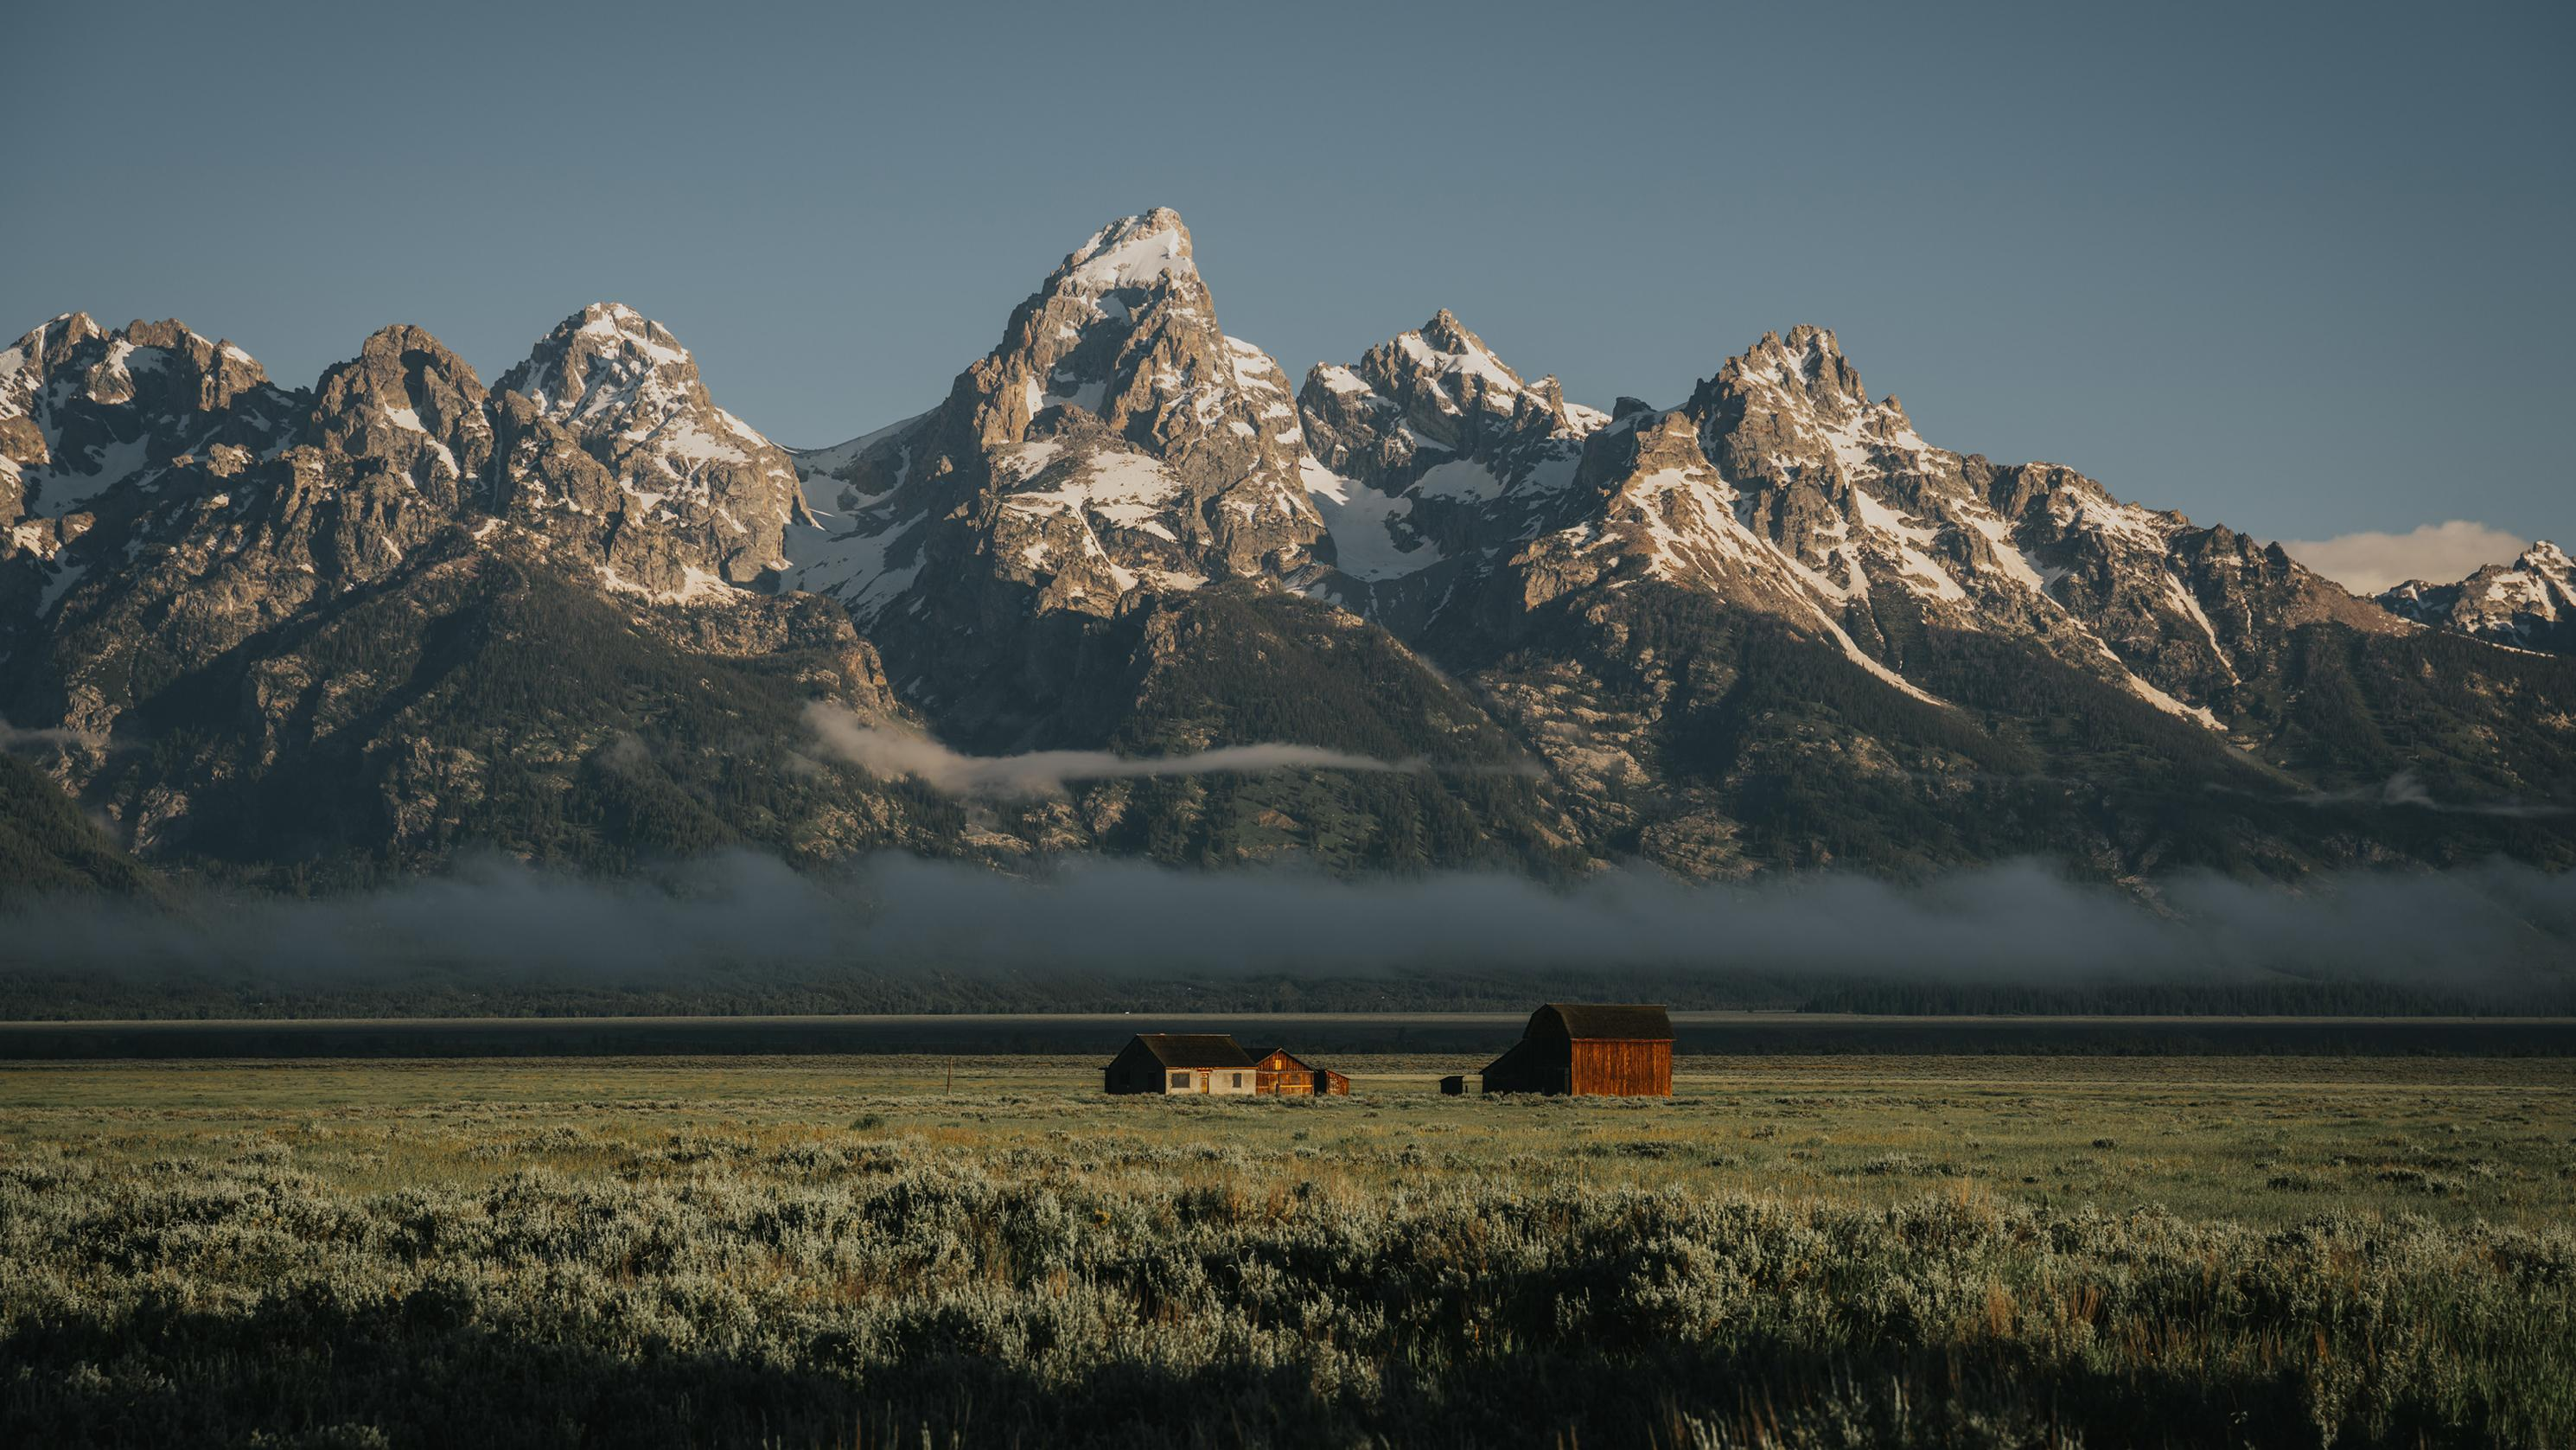
\includegraphics[width=\textwidth]{images/1.jpg}
    \caption{1}
  \end{minipage}
  \begin{minipage}{0.49\textwidth}
    \centering
    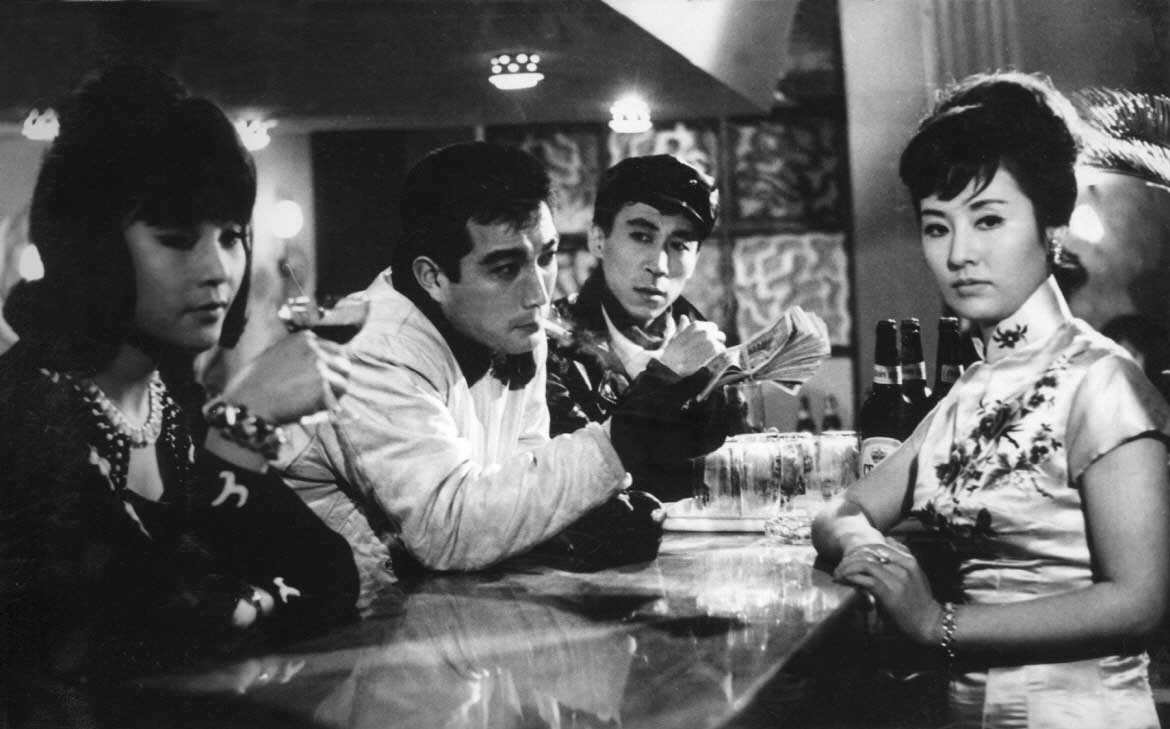
\includegraphics[width=\textwidth]{images/2.jpg}
    \caption{2}
  \end{minipage}
  \end{figure}
\end{minted}


\newpage

  
\section{minted  \textcolor{green}{\faIcon{github}} \textcolor{blue}{\faIcon{code}} \faIcon{university} \textcolor{cyan}{\faIcon{google-plus}} \faIcon{at}}

\begin{texcode}
  % sudo pip3 install pygments
  % -shell-escape

  \documentclass[letterpaper, 10pt]{article}
  \usepackage{minted}
  \usepackage{xcolor}
  \usepackage{fontawesome5} % \textcolor{green}{\faIcon{github}}

  \usemintedstyle{xcode} % pygmentize -L styles [xcode, github-dark]
  

  % Custom Code Environments
  \newminted{tex}{
    gobble=2,
    linenos,
    mathescape,
    numbersep=5pt,
    frame=single,
    baselinestretch=1.2,
    fontsize=\normalsize, % huge, LARGE, large, normalsize, small, footnotesize, scriptsize, tiny
    highlightcolor=yellow!50,
    highlightlines={1,3},
    bgcolor=bg,
    breaklines,
  }

  \begin{document}

  % \begin{Customcode}
  \begin{minted}[
      encoding=utf8,
      linenos,
      gobble=2,
      mathescape,
      numbersep=5pt,
      frame=single,
      framesep=2mm,
      baselinestretch=1.2,
      fontsize=\large, % huge, LARGE, large, normalsize, small, footnotesize, scriptsize, tiny
      highlightcolor=yellow!50,
      highlightlines={1,3},
      bgcolor=bg,
      breaklines]{tex}
    ...
  \end{minted}
  % \end{Customcode}

  \end{document}
\end{texcode}

\newpage

  \section{tabularray \textcolor{green}{\faIcon{github}} \textcolor{blue}{\faIcon{code}} \faIcon{university} \textcolor{cyan}{\faIcon{google-plus}} \faIcon{at}}

\begin{minted}[
  encoding=utf8,
  linenos,
  gobble=2,
  mathescape,
  numbersep=5pt,
  frame=single,
  framesep=2mm,
  baselinestretch=1.2,
  fontsize=\normalsize, % huge, LARGE, large, normalsize, small, footnotesize, scriptsize
  highlightcolor=cyan!50,
  highlightlines={2,27},
  breaklines]{tex}
  \documentclass[letterpaper, 10pt]{article}
  \usepackage{tabularray}
  \usepackage{xcolor}
  \usepackage{chngcntr} % resort

  \definecolor{mygrey}{RGB}{128,128,128}
  \definecolor{myteal}{RGB}{0,128,128}
  \definecolor{mypink}{RGB}{250,218,221}

  \NewTblrEnviron{mytblr}
  \SetTblrOuter[mytblr]{long}
  \SetTblrInner[mytblr]{
    width = 0.99\linewidth,
    rowhead = 1,
    verb,
    row{odd} = {bg=mypink}, 
    row{1}   = {bg=myteal, fg=white},
  }
  \SetTblrStyle{caption-tag}{red2}
  \SetTblrStyle{firstfoot}{fg=blue2}
  \SetTblrStyle{firsthead}{font=\bfseries}

  \UseTblrLibrary{counter}
  \newcounter{mycnta}
  \newcommand{\mycnta}{\stepcounter{mycnta}\arabic{mycnta}}
  % resort on Page
  \counterwithin{mycnta}{page}
  \renewcommand\themycnta{\arabic{mycnta}}

  \NewTableCommand\myhline{\hline[0.2em,black]}
  
  \begin{document}

  \begin{mytblr}[
      caption = {caption Name},
    ]{
      colspec = {|l|X[2.8]|X[2.8]|X[2.8]|X[2.8]|},
      }
      \myhline
      \SetRow{c} ID & column1  & column2  & column3  & column4 \\
      \myhline
      \mycnta & text1 & text2 & test3 & test 4 \\
      ...
      \myhline
  \end{mytblr}

  \end{document}
\end{minted}

\newpage


  \end{document}
\end{minted}

\newpage



\section{fontawesome5 \textcolor{green}{\faIcon{github}} \textcolor{blue}{\faIcon{code}} \faIcon{university} \textcolor{cyan}{\faIcon{google-plus}} \faIcon{at}}

\begin{minipage}[t]{.5\linewidth}
\begin{tabular}{rp{.75\linewidth}}
	\baselineskip=20pt
	\email{} :     & \href{2353442022@qq.com}{2353442022@qq.com}\\
	\www{} : &\href{https://fontawesome.com/v5/search}{https://fontawesome.com/v5/search}
\end{tabular}
\end{minipage}
\begin{minipage}[t]{.5\linewidth}
\begin{tabular}{rl}
	\gh{} : & \href{https://github.com/lcdse7en}{https://github.com/lcdse7en}\\
	\gitee{} : &\href{https://gitee.com/se7enlcd}{https://gitee.com/se7enlcd}
\end{tabular}
\end{minipage}

\begin{minted}[
  encoding=utf8,
  linenos,
  gobble=2,
  mathescape,
  numbersep=5pt,
  frame=single,
  framesep=2mm,
  baselinestretch=1.2,
  fontsize=\normalsize, % huge, LARGE, large, normalsize, small, footnotesize, scriptsize
  highlightcolor=cyan!50,
  highlightlines={6,8},
  breaklines]{tex}
  \documentclass[letterpaper, 10pt]{article}
  \usepackage{fontawesome5}

  \begin{document}

  \faIcon{tint}

  \textcolor{red}{\faIcon{tint}}

  \end{document}

\end{minted}


\begin{mytblr}[
    caption = {Fontawesome5 Icons},
  ]{
    colspec={|l|X[2.8]|X[2.8]|l|X[2.8]|X[2.8]|X[2.8]|},
    }
    \myhline
    \SetRow{c} ID & Icon Name & Show            & ID         & Icon Name    & Show                  \\
    \myhline
    \mycnta & yin-yang    & \faIcon{yin-yang}     & \mycnta    & transgender  & \faIcon{transgender}  \\
    \mycnta & yen-sign    & \faIcon{yen-sign}     & \mycnta    & toggle-on    & \faIcon{toggle-on}    \\
    \mycnta & video       & \faIcon{video}        & \mycnta    & terminal     & \faIcon{terminal}     \\
    \mycnta & user-secret & \faIcon{user-secret}  & \mycnta    & tag          & \faIcon{tag}          \\
    \mycnta & store       & \faIcon{store}        & \mycnta    & share        & \faIcon{share}       \\
    \mycnta & phone-volume& \faIcon{phone-volume} & \mycnta    & pen-nib      & \faIcon{pen-nib}     \\
    \mycnta & smoking-ban & \faIcon{smoking-ban}  & \mycnta    & magnet       & \faIcon{magnet}      \\
    \mycnta & smoking     & \faIcon{smoking}      & \mycnta    & landmark     & \faIcon{landmark}    \\
    \mycnta & id-card     & \faIcon{id-card}    & \mycnta      & heart        & \faIcon{heart}       \\
    \mycnta & code     & \faIcon{code}    & \mycnta      & clock        & \faIcon{clock}       \\
    \mycnta & clone     & \faIcon{clone}    & \mycnta      & check        & \faIcon{check}       \\
    \mycnta & youtube     & \faIcon{youtube}    & \mycnta      & weixin        & \faIcon{weixin}       \\
    \mycnta & weibo     & \faIcon{weibo}    & \mycnta      & whatsapp        & \faIcon{whatsapp}       \\
    \mycnta & python     & \faIcon{python}    & \mycnta      & qq        & \faIcon{qq}       \\
    \mycnta & google-plus     & \faIcon{google-plus}    & \mycnta      & github        & \faIcon{github}       \\
    \mycnta & chrome     & \faIcon{chrome}    & \mycnta      & tint        & \faIcon{tint}       \\
    \mycnta & chart-line     & \faIcon{chart-line}    & \mycnta      &         &        \\
    \mycnta &             &             & \mycnta      &         &        \\
    \mycnta &             &             & \mycnta      &         &        \\
    \mycnta &             &             & \mycnta      &         &        \\
    \mycnta &             &             & \mycnta      &         &        \\
    \mycnta &             &             & \mycnta      &         &        \\
    \mycnta &             &             & \mycnta      &         &        \\
    \mycnta &             &             & \mycnta      &         &        \\
    \mycnta &             &             & \mycnta      &         &        \\
    \myhline 
\end{mytblr}

\newpage

\section{graphicx \textcolor{green}{\faIcon{github}} \textcolor{blue}{\faIcon{code}} \faIcon{university} \textcolor{cyan}{\faIcon{google-plus}} \faIcon{at}}


\begin{minted}[
  encoding=utf8,
  linenos,
  gobble=2,
  mathescape,
  numbersep=5pt,
  frame=single,
  framesep=2mm,
  baselinestretch=1.2,
  fontsize=\normalsize, % huge, LARGE, large, normalsize, small, footnotesize, scriptsize
  highlightcolor=cyan!50,
  highlightlines={7,12},
  breaklines]{tex}
  \usepackage{graphicx}

  \begin{figure}[hbt!]
  \centering
  \begin{minipage}{0.49\textwidth}
    \centering
    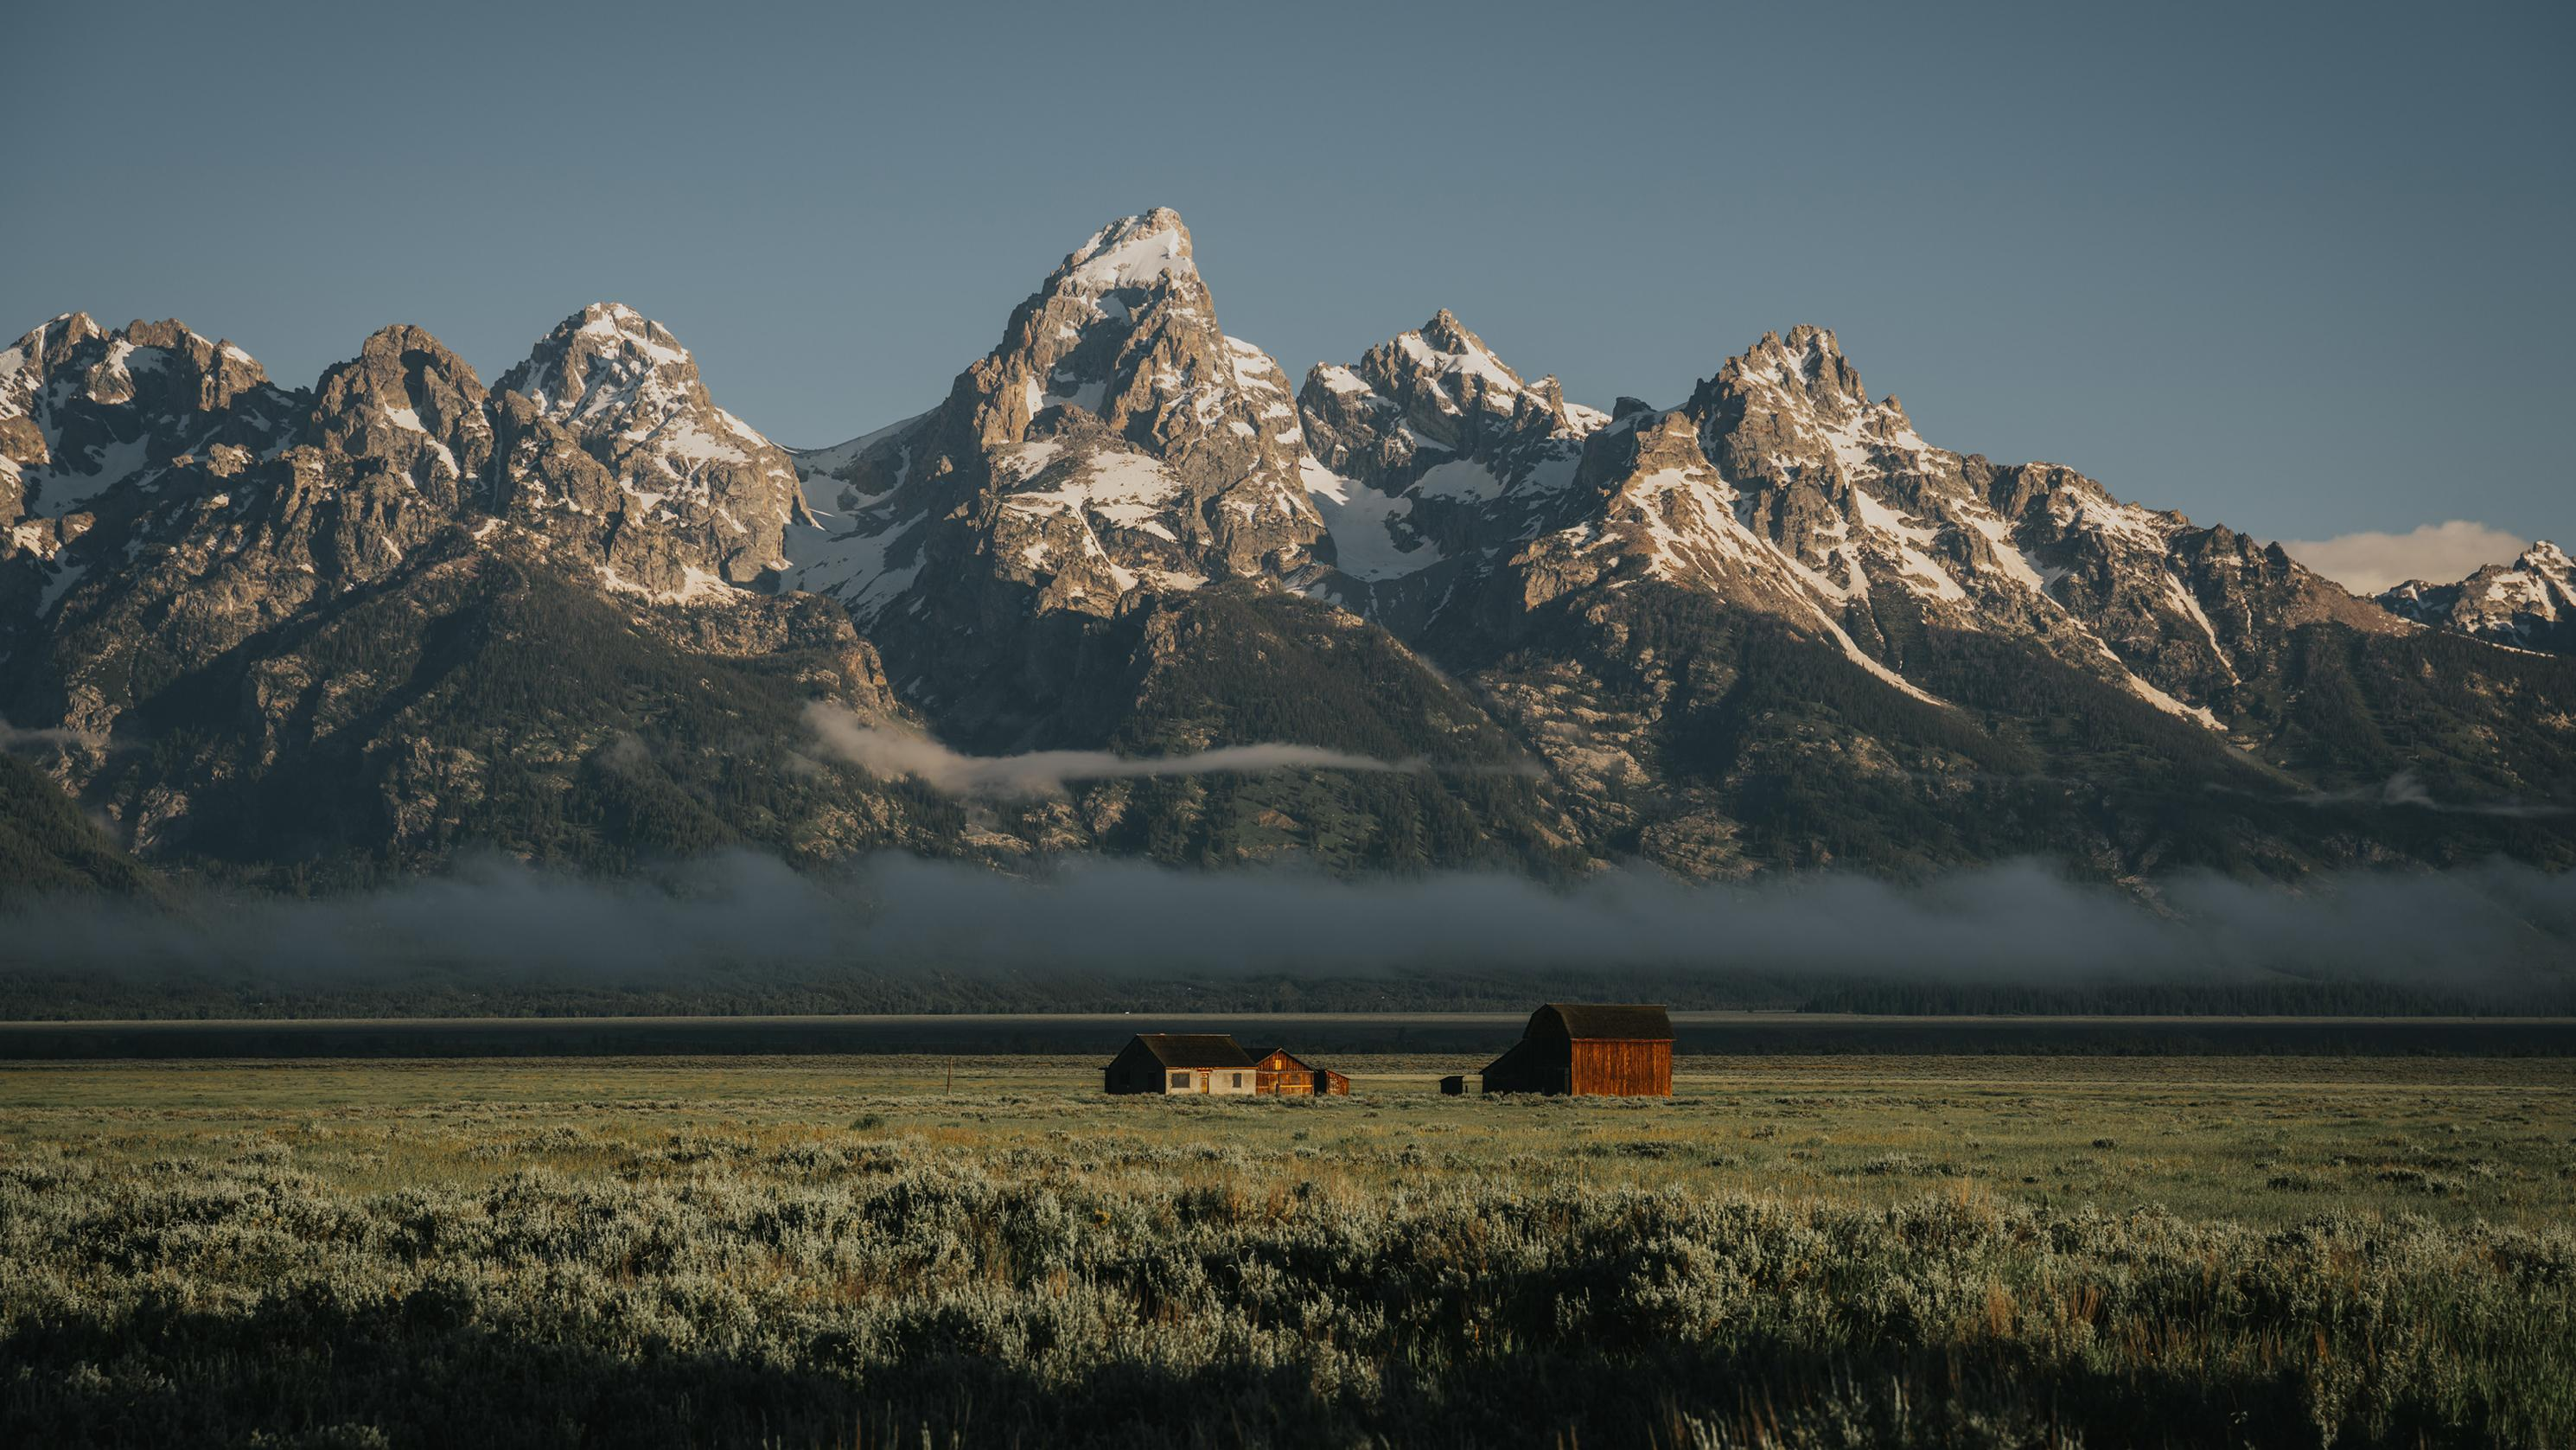
\includegraphics[width=\textwidth]{images/1.jpg}
    \caption{1}
  \end{minipage}
  \begin{minipage}{0.49\textwidth}
    \centering
    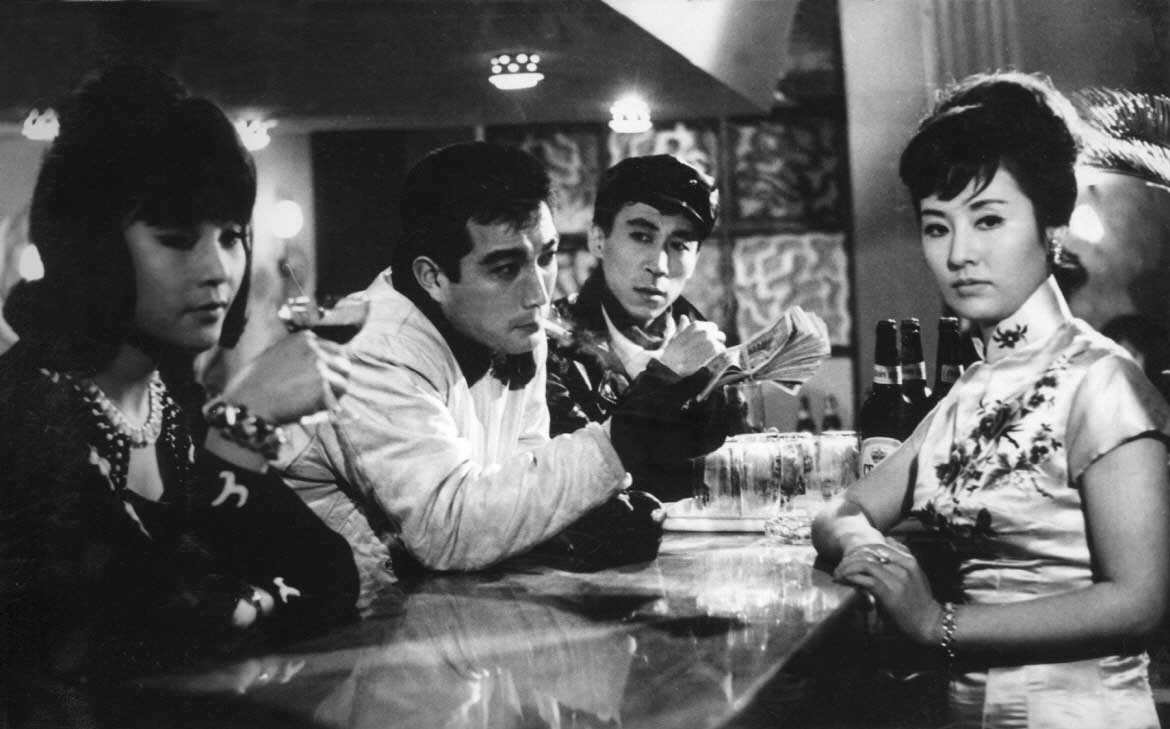
\includegraphics[width=\textwidth]{images/2.jpg}
    \caption{2}
  \end{minipage}
  \end{figure}
\end{minted}


\newpage


\section{minted  \textcolor{green}{\faIcon{github}} \textcolor{blue}{\faIcon{code}} \faIcon{university} \textcolor{cyan}{\faIcon{google-plus}} \faIcon{at}}

\begin{texcode}
  % sudo pip3 install pygments
  % -shell-escape

  \documentclass[letterpaper, 10pt]{article}
  \usepackage{minted}
  \usepackage{xcolor}
  \usepackage{fontawesome5} % \textcolor{green}{\faIcon{github}}

  \usemintedstyle{xcode} % pygmentize -L styles [xcode, github-dark]
  

  % Custom Code Environments
  \newminted{tex}{
    gobble=2,
    linenos,
    mathescape,
    numbersep=5pt,
    frame=single,
    baselinestretch=1.2,
    fontsize=\normalsize, % huge, LARGE, large, normalsize, small, footnotesize, scriptsize, tiny
    highlightcolor=yellow!50,
    highlightlines={1,3},
    bgcolor=bg,
    breaklines,
  }

  \begin{document}

  % \begin{Customcode}
  \begin{minted}[
      encoding=utf8,
      linenos,
      gobble=2,
      mathescape,
      numbersep=5pt,
      frame=single,
      framesep=2mm,
      baselinestretch=1.2,
      fontsize=\large, % huge, LARGE, large, normalsize, small, footnotesize, scriptsize, tiny
      highlightcolor=yellow!50,
      highlightlines={1,3},
      bgcolor=bg,
      breaklines]{tex}
    ...
  \end{minted}
  % \end{Customcode}

  \end{document}
\end{texcode}

\newpage

\section{tabularray \textcolor{green}{\faIcon{github}} \textcolor{blue}{\faIcon{code}} \faIcon{university} \textcolor{cyan}{\faIcon{google-plus}} \faIcon{at}}

\begin{minted}[
  encoding=utf8,
  linenos,
  gobble=2,
  mathescape,
  numbersep=5pt,
  frame=single,
  framesep=2mm,
  baselinestretch=1.2,
  fontsize=\normalsize, % huge, LARGE, large, normalsize, small, footnotesize, scriptsize
  highlightcolor=cyan!50,
  highlightlines={2,27},
  breaklines]{tex}
  \documentclass[letterpaper, 10pt]{article}
  \usepackage{tabularray}
  \usepackage{xcolor}
  \usepackage{chngcntr} % resort

  \definecolor{mygrey}{RGB}{128,128,128}
  \definecolor{myteal}{RGB}{0,128,128}
  \definecolor{mypink}{RGB}{250,218,221}

  \NewTblrEnviron{mytblr}
  \SetTblrOuter[mytblr]{long}
  \SetTblrInner[mytblr]{
    width = 0.99\linewidth,
    rowhead = 1,
    verb,
    row{odd} = {bg=mypink}, 
    row{1}   = {bg=myteal, fg=white},
  }
  \SetTblrStyle{caption-tag}{red2}
  \SetTblrStyle{firstfoot}{fg=blue2}
  \SetTblrStyle{firsthead}{font=\bfseries}

  \UseTblrLibrary{counter}
  \newcounter{mycnta}
  \newcommand{\mycnta}{\stepcounter{mycnta}\arabic{mycnta}}
  % resort on Page
  \counterwithin{mycnta}{page}
  \renewcommand\themycnta{\arabic{mycnta}}

  \NewTableCommand\myhline{\hline[0.2em,black]}
  
  \begin{document}

  \begin{mytblr}[
      caption = {caption Name},
    ]{
      colspec = {|l|X[2.8]|X[2.8]|X[2.8]|X[2.8]|},
      }
      \myhline
      \SetRow{c} ID & column1  & column2  & column3  & column4 \\
      \myhline
      \mycnta & text1 & text2 & test3 & test 4 \\
      ...
      \myhline
  \end{mytblr}

  \end{document}
\end{minted}

\newpage

% % \begin{minipage}[t][][t]{.6\textwidth}
%   \begin{texcode}
%   \usepackage[customcolors,shade]{hf-tikz}
%   \usepackage{tkz-euclide}

%   \begin{tikzpicture}
%     \tkzDefPoints{0/0/A,4/0/B,3/3/C}
%     \tkzDrawPoints(A,B,C)
%     \tkzLabelPoints(A,B,C)
%     \tkzDrawPolygon(A,B,C) 
%     \tkzLabelSegment[above left](A,C){$\sqrt{13}$}
%     \tkzFillAngle[size=0.5cm, right color=white, left color=red!50](C,B,A)
%     \tkzLabelAngle[pos=1](C,B,A){$26.6^\circ$}
%   \end{tikzpicture}
%   \end{texcode}
% \end{minipage}
% \quad
% \begin{minipage}[t][][b]{.3\textwidth}
%     \begin{tikzpicture}
%       \tkzDefPoints{0/0/A,4/0/B,3/3/C}
%       \tkzDrawPoints(A,B,C)
%       \tkzLabelPoints(A,B,C)
%       \tkzDrawPolygon(A,B,C) 
%       \tkzLabelSegment[above left](A,C){$\sqrt{13}$}
%       \tkzFillAngle[size=0.5cm, right color=white, left color=red!50](C,B,A)
%       \tkzLabelAngle[pos=1](C,B,A){$26.6^\circ$}
%     \end{tikzpicture}
% \end{minipage}

\section{tkz-euclide \textcolor{green}{\faIcon{github}} \textcolor{blue}{\faIcon{code}} \faIcon{university} \textcolor{cyan}{\faIcon{google-plus}} \faIcon{at}}

\begin{tikzpicture}[scale=3]
\tikzset{
arr/.style={postaction=decorate,
decoration={markings,
mark=at position 1 with {\arrow[thick]{#1}}
}}}
\pgfkeys{/pgf/number format/.cd,fixed,precision=2}
\tkzDefPoints{-1/0/A',0/0/A, 1/0/B,2/0/C}
\tkzDefPoints{0/0.5/E,1/0.5/F,2/0.5/G}

\tkzDrawSegment[color=red,thin, arr=stealth](A,C)
\tkzDrawSegment[color=red,thin, arr=stealth](A,E)
\tkzDrawSegment[color=red,thin, arr=stealth](B,F)
\tkzDrawSegment[color=red,thin, arr=stealth](C,G)
\tkzDrawSegment[style=dashed, color=orange](A',A)
\tkzDrawPoints(A',A,B,C)
  \tkzLabelPoints[teal,above left](A)
\tkzDrawLines[add=0 and .5](A,C)
\tkzCalcLength[cm](A,B)\tkzGetLength{ABl}
\tkzCalcLength[cm](B,C)\tkzGetLength{BCl}
% \tkzDrawSegment[dim={\pgfmathprintnumber\ABl,-6pt,transform shape}](A,B)
\tkzDrawSegment[dim={\pgfmathprintnumber\ABl,-6pt,transform shape}](A,B)
\tkzDrawSegment[dim={\pgfmathprintnumber\BCl,-6pt,transform shape}](B,C)
\end{tikzpicture}




\end{document}






